\documentclass{beamer}

\usepackage[latin1]{inputenc}
\usepackage{algorithmic}
\usepackage{amsmath}
\usepackage{graphicx}
\usepackage{verbatim}
\usepackage{hyperref}

\title{Super-Resolution From a Single Image}
\author{Geoffrey Ulman}
\date{April 21, 2012}
\begin{document}

%%%%%%%%%%%%%%%%%%%%%%%%%%%%%%%%%%%%%%%%%%%%%%%%%%%%

\begin{frame}
\titlepage
\end{frame}

%%%%%%%%%%%%%%%%%%%%%%%%%%%%%%%%%%%%%%%%%%%%%%%%%%%%

\begin{frame}{Original Paper}

Super-Resolution From a Single Image

\vspace{1cm}

\emph{Daniel Glasner, Shai Bagon, Michal Irani}

\vspace{1cm}

\url{http://www.wisdom.weizmann.ac.il/~vision/SingleImageSR.html}

\end{frame}

%%%%%%%%%%%%%%%%%%%%%%%%%%%%%%%%%%%%%%%%%%%%%%%%%%%%

\begin{frame}{Multiple Frame Super-Resolution}

\begin{figure}
\centering
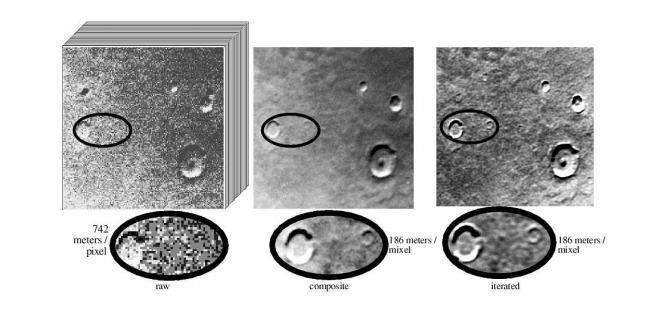
\includegraphics[width=1.0\textwidth]{presentation_screen1.png}
\caption{Multiple images of the same scene with sub-pixel shifts\footnote[1]{\url{http://www.robots.ox.ac.uk/~elle/pubs/elle-thesis.pdf}}}
\end{figure}

\end{frame}

%%%%%%%%%%%%%%%%%%%%%%%%%%%%%%%%%%%%%%%%%%%%%%%%%%%%

\end{document}
